\subsection{Problem Statement}
\label{sec:statement}

\subsubsection{Task Definition}
The input is a casual video featuring a single person. 2D pose sequences are extracted using Pose Extractors \cite{openpose2020,alphapose2022}, resulting in a tensor $p \in \mathbb{R}^{S \times J_{2d} \times C_{in}}$, where $S = 150$ frames (5 seconds at 30 FPS), $J_{2d} = 17$ joints (COCO format), and $C_{in} = 3$ (x, y, confidence). Missing or low-confidence joints are masked to ensure reliable conditioning. The objective is to generate a corresponding 3D motion sequence $M \in \mathbb{R}^{S \times (J_{3d} \cdot C + 4 + 3)}$, comprising:
\begin{itemize}
    \item Flattened joint rotations $R \in \mathbb{R}^{J_{3d} \times C}$ with $J_{3d} = 24$ joints in 6D rotation space ($C = 6$),
    \item Foot contact labels $f \in \{0,1\}^4$ for ankles and feet,
    \item Root position $t \in \mathbb{R}^3$ (global translation).
\end{itemize}
The output preserves the stylistic qualities of the input video and is suitable for downstream physics-based simulation and animation tasks.

\subsubsection{Dataset}
The AIST++ dataset provides the training corpus, containing 1,408 sequences of 3D dance motions, multi-view videos, and synchronized annotations~\cite{aist2021}. Motion sequences are stored as SMPL pose parameters ($\text{smpl\_poses} \in \mathbb{R}^{N \times 24 \times 3}$) and global translation ($\text{smpl\_trans} \in \mathbb{R}^{N \times 3}$). 2D keypoints ($\text{keypoints2d} \in \mathbb{R}^{9 \times N \times 17 \times 3}$) represent nine calibrated camera views, $N$ frames, 17 COCO-format joints, and per-joint (x, y, confidence) values in pixel coordinates at 1920×1080 resolution. Raw and optimized 3D keypoints ($\text{keypoints3d} \in \mathbb{R}^{N \times 17 \times 3}$) are provided, with timestamps annotated at 60 FPS. The dataset covers 10 dance genres and hundreds of choreographies, making it suitable for training models to generalize across motion categories and camera conditions~\cite{aist2021}.

\begin{figure}[htb]
    \centering
    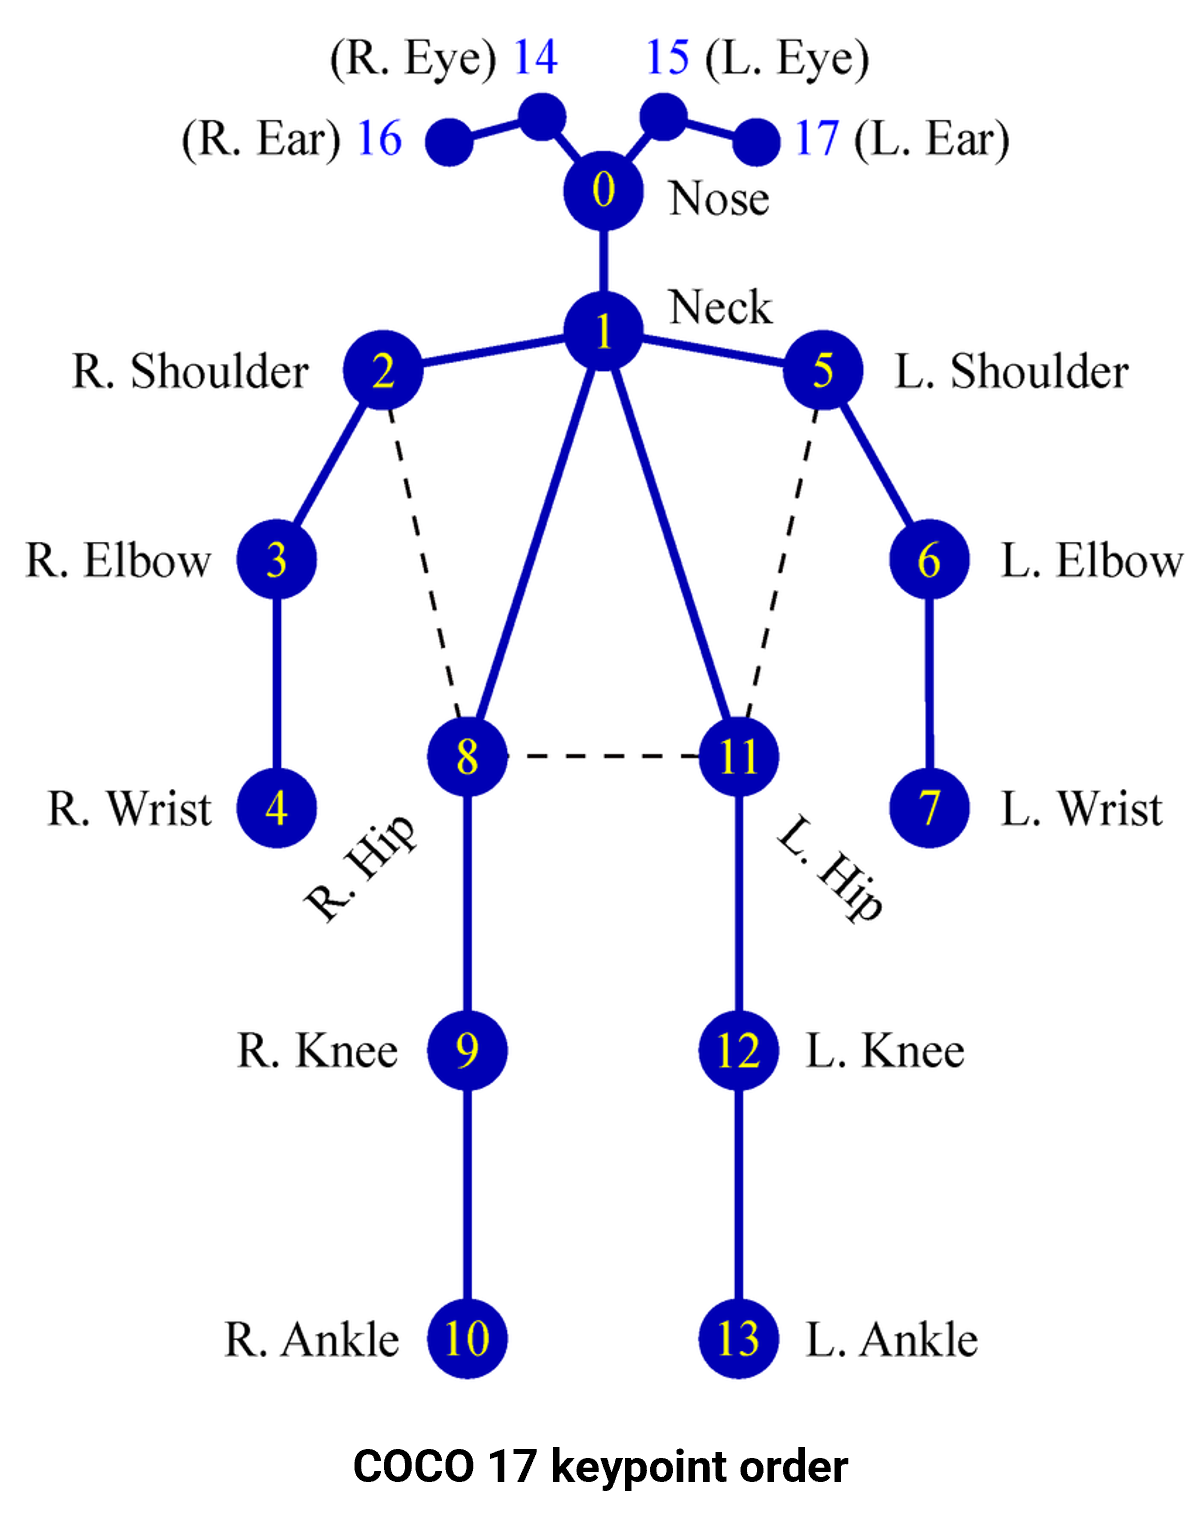
\includegraphics[width=0.5\textwidth]{Pictures/keypoints.png}
    \caption{Human Skeleton's COCO 17-Keypoint Order.}
    \label{fig:keypoints}
\end{figure}

\subsubsection{Pose Estimators}
The 2D skeletons used for conditioning are extracted using OpenPose~\cite{openpose2020} and AlphaPose~\cite{alphapose2022}. Both models provide per-joint confidence scores, which are used to mask out unreliable detections. In multi-view scenarios, the highest-confidence detection per joint is selected or aggregated through a lightweight learned module. Optional temporal smoothing can reduce jitter, but is applied cautiously to avoid removing meaningful micro-motions. Occlusion and rapid camera motion are common in casual footage; the pipeline treats pose estimates as noisy and designs both the denoiser and auxiliary losses to be resilient to such errors~\cite{vimo2024}.

\begin{figure}[htb]
    \centering
    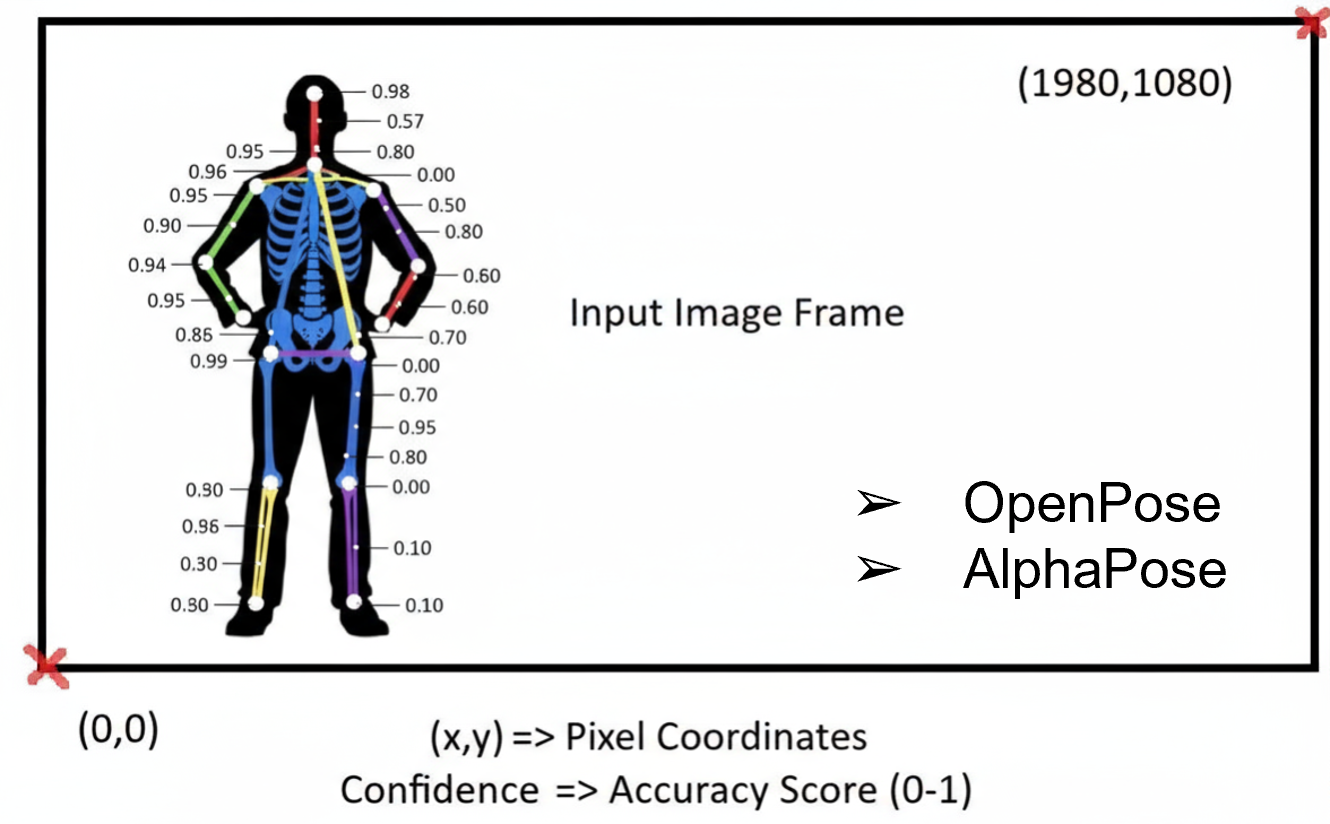
\includegraphics[width=0.75\textwidth]{Pictures/posedata.png}
    \caption{Representation of the Pose Estimator's Output}
    \label{fig:posedata}
\end{figure}

\subsubsection{Preprocessing}
Raw AIST++~\cite{aist2021} sequences are resampled from 60 FPS to 30 FPS by selecting every second frame. Sequences are partitioned into non-overlapping clips of 150 frames (5 seconds). The conditioning tensor $\text{cond\_2d}$ retains shape $V \times 150 \times 17 \times 3$ for $V$ views. Ground-truth 3D motion $\text{m3d\_gt}$ is constructed per clip as $150 \times 151$, encoding 24 joints in 6D rotation format (144 dimensions), 4 foot contact labels, and 3 root position values. Sequences listed in $\text{ignore\_list.txt}$ are omitted. SMPL axis-angle rotations are converted to 6D using orthogonalization~\cite{6drot2020}. Foot contact labels are pre-computed from foot and toe vertical velocities near zero. The 2D pose coordinates are given in image pixels, which are not directly meaningful for 3D motion generation. To address this, the preprocessing normalizes the poses by centering them relative to the root joint, ensuring the model conditions on relative joint positions rather than absolute image coordinates. This step is crucial for generalizing across different camera views and video scales. The resulting tensors feed the diffusion training loop directly, ensuring temporal coherence and compatibility with the model architecture~\cite{vimo2024}.
